% 1.1.Download.tex
%	Last update: 2020/02/10 F.Kanehori
%\newpage
\subsection{ダウンロード}
\label{subsec:Download}
\parindent=0pt

\SprLib はGitHubで管理されており、
次のURLからダウンロードすることができます。
\bf{以下、ダウンロードするディレクトリを\SprTop{}として説明を進めます。}

\CmndLine{%
	> chdir C:/Springhead\\
	> git clone --recurse-submodules\Cont\\
	\Hskip{100pt}https://github.com/sprphys/Springhead
}{command-1-1-a.eps}{DownloadTree1}
\medskip

デフォルトでpythonが利用できる環境であればサブモジュールbuildtoolは必要ありません。
また、外部パッケージboost, glew, glut, glui を別途インストールして使用するのであれば
サブモジュールdependencyは必要ありません。
そのような場合には、次のようにしてサブモジュールを選択してください。

\CmndLine{%
	> chdir C:/Springhead\\
	> git clone https://github.com/sprphys/Springhead\\
	> git submodule update --init --checkout buildtool\\
	> git submodule update --init --checkout dependency
}{command-1-1-b.eps}{DownloadTree2}

\medskip
Windows exploreならば右クリックでGUIが利用できます。
Git clone の画面で recursiveにチェックを入れると
サブモジュールも一緒にダウンロードできます。

\begin{narrow}[15pt]
	\begin{figure}[h]
	\begin{center}
	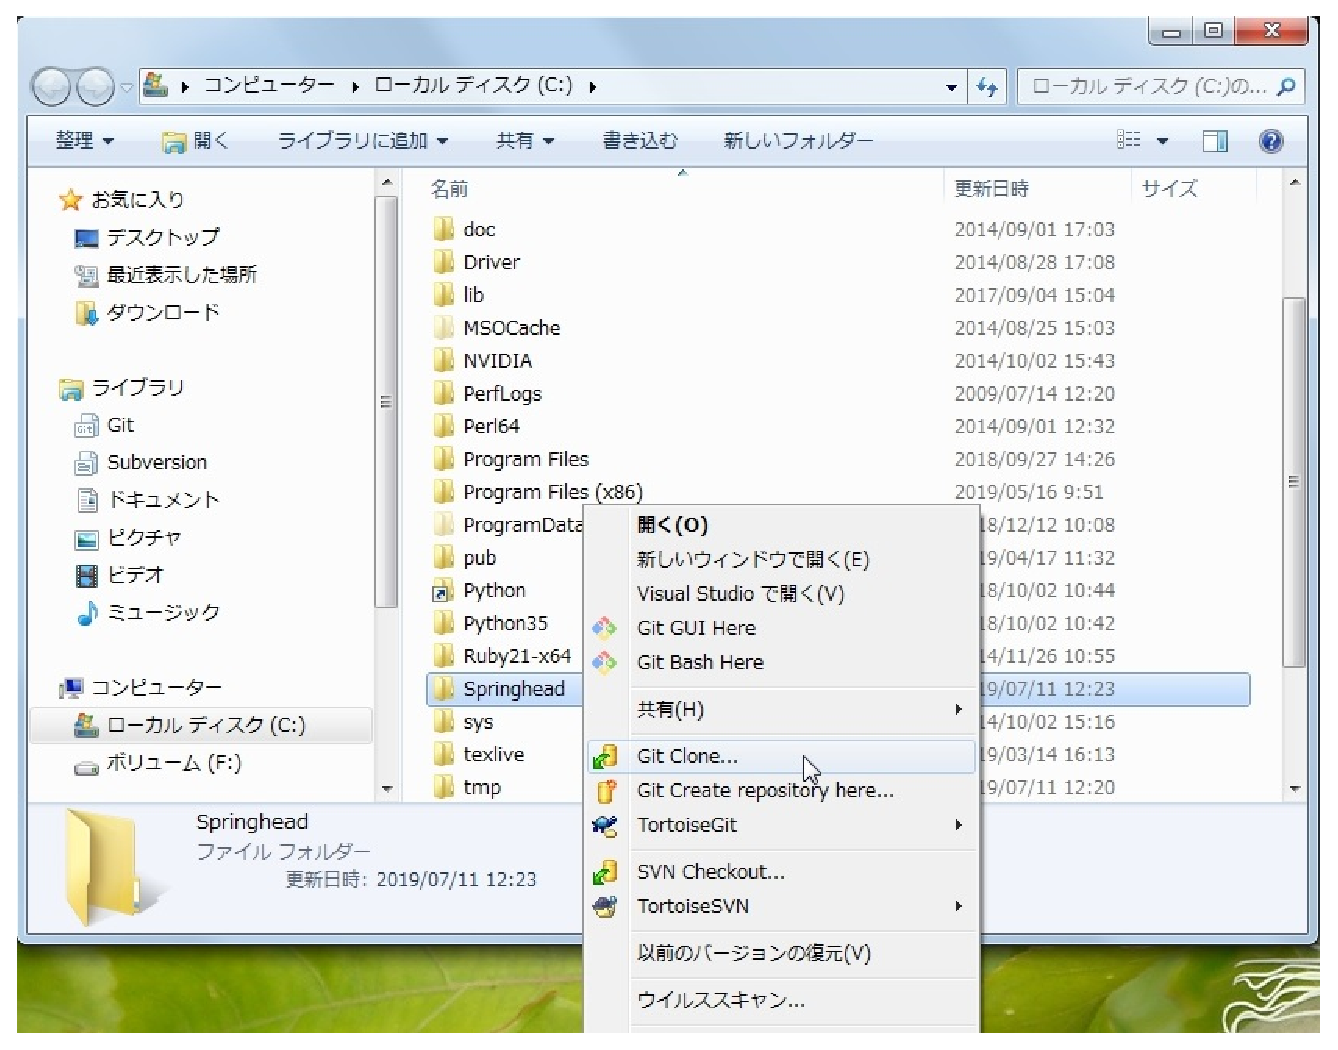
\includegraphics[width=0.5\textwidth]{fig/SpringheadClone1.eps}
	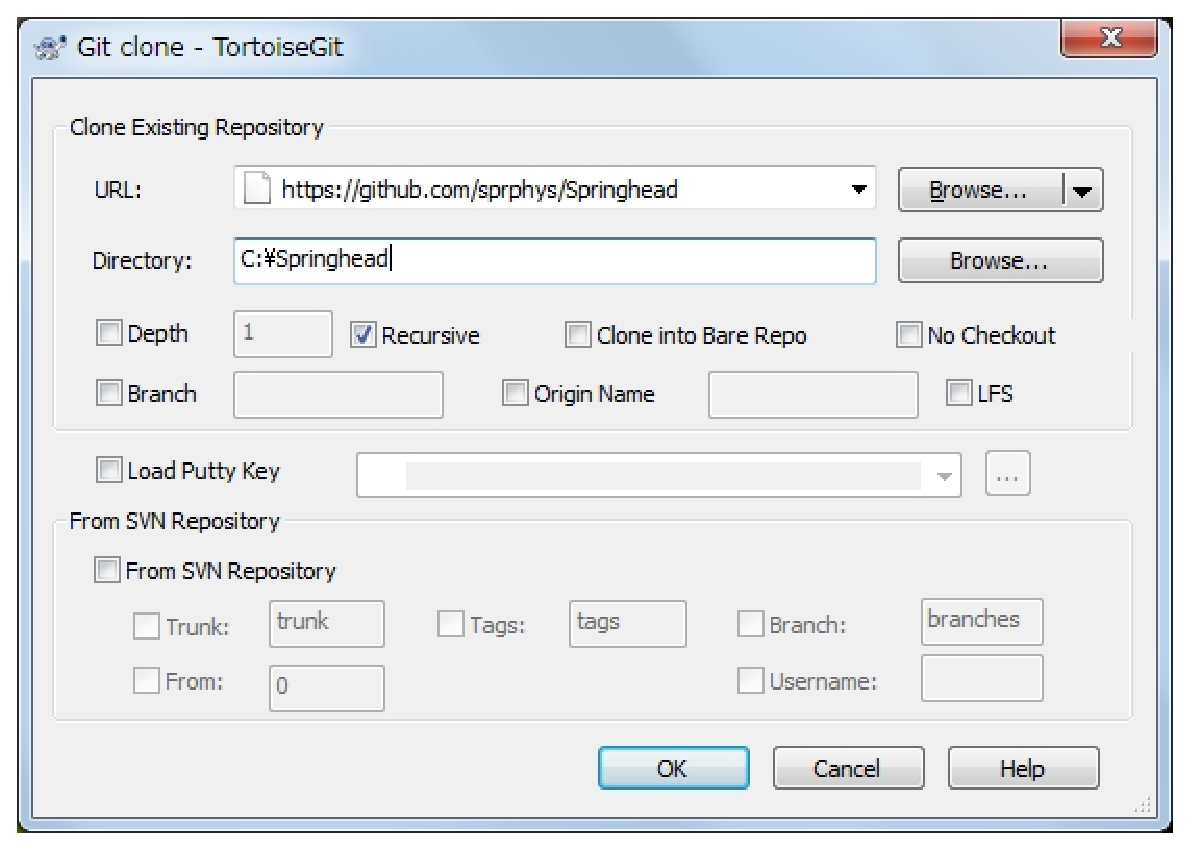
\includegraphics[width=0.4\textwidth]{fig/SpringheadClone2.eps}
	\end{center}
	\caption{Springheadダウンロード}
	\label{fig:SpringheadClone}
	\end{figure}
\end{narrow}

\Important{%
	サブモジュールを導入するのに必要なディスク容量は、
	buildtoolが約32MB、dependencyが約550MBです。}

\bigskip
% end 1.1.Download.tex
